\documentclass[11pt, oneside]{article} 
\usepackage{geometry}
\geometry{letterpaper} 
\usepackage{graphicx}
	
\usepackage{amssymb}
\usepackage{amsmath}
\usepackage{parskip}
\usepackage{color}
\usepackage{hyperref}

\graphicspath{{/Users/telliott_admin/Dropbox/Tex/png/}}
% \begin{center} 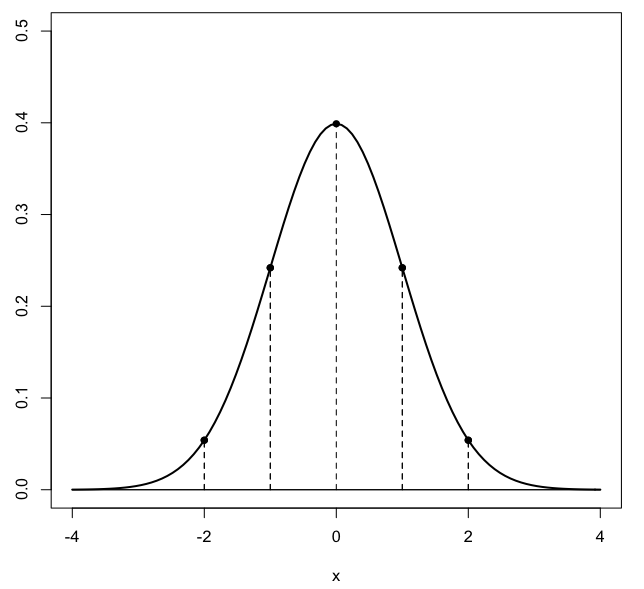
\includegraphics [scale=0.4] {gauss3.png} \end{center}

\title{Intermediate Value Theorem}
\date{}

\begin{document}
\maketitle
\Large
\subsection*{Bolzano's Theorem}

We prove this as a preliminary to proof of the IVT.

If $f$ is continuous on $[a,b]$ and $f(a) < 0 < f(b)$ then there is some $x$ in $[a,b]$ such that $f(x) = 0$.
\begin{center} 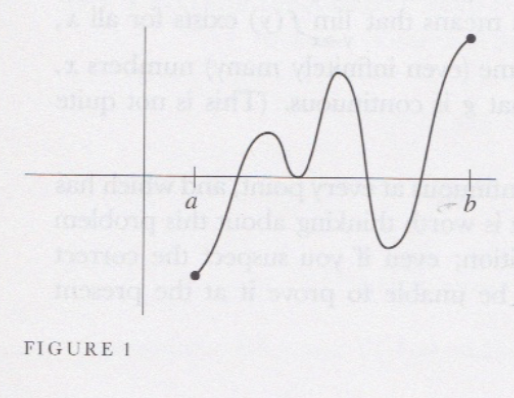
\includegraphics [scale=0.4] {spivak1.png} \end{center}

\subsection*{Proof}
$\bullet$  Let $\mathbf{S}$ be the set of all $x \in [a,b]$ such that $f(x) \le 0$.  

$\bullet$  $\mathbf{S}$ is non-empty ($\mathbf{S} \ne \varnothing$) since $a \in \mathbf{S}$.  

$\bullet$  Since $f(b) > 0$, $b \notin \mathbf{S}$, and since the relevant interval is $[a,b]$, $b$ is larger than all members of $\mathbf{S}$, and so $b$ is an upper bound of $\mathbf{S}$.
 
$\bullet$  Therefore, by \textbf{completeness}, there exists a least upper bound or supremum of $\mathbf{S}$. 

$\bullet$  Define $c$ to be that supremum.  Since $f(x)$ is continuous, $\lim_{x \rightarrow c} f(x) = f(c)$.

\noindent\rule{2cm}{0.4pt}

One of three things is true:  $f(c) > 0, f(c) < 0$ or $f(c) = 0$.  We claim that $f(c) = 0$.  The proof is by contradiction.  

Suppose $f(c) > 0$.

$\bullet$  We define $\epsilon_1 = f(c)/2$.  Then $\epsilon_1$ is positive and $2 \epsilon_1 = f(c) > 0$.

$\bullet$  By the definition of the limit, there exists $\delta_1$, such that for all $0 < |x - c| < \delta_1$ it is true that
\[ |f(x) - f(c)| < \epsilon_1 \]

$\bullet$  Then (see the triangle inequality write-up)
\[ -\epsilon_1 < f(x) - f(c) < \epsilon_1 \]
\[ -\epsilon_1 < f(x) - 2 \epsilon_1 < \epsilon_1 \]
\[ \epsilon_1 < f(x) < 3 \epsilon_1 \]

so this implies that $f(x) > 0$ everywhere in the interval $c - \delta_1 < x < c + \delta_1$.

$\bullet$  It would appear that we have found a smaller upper bound for the set $\mathbf{S}$ in the interval $[c - \delta_1,c]$.  But $c$ is a least upper bound, so this is a contradiction.

We conclude that $f(c) > 0$ is impossible.

\noindent\rule{2cm}{0.4pt}

Suppose $f(c) < 0$.

$\bullet$  We can define $\epsilon_2 = -f(c)/2$.  Then $\epsilon_2 > 0$ and $-f(c) = 2 \epsilon_2$.

$\bullet$  By the definition of the limit, there exists $\delta_2$, such that for all $0 < |x - c| < \delta_2$ it is true that
\[ |f(x) - f(c)| < \epsilon_2 \]

$\bullet$  Then
\[ -\epsilon_2 < f(x) - f(c) < \epsilon_2 \]
We have $-f(c) = 2 \epsilon_2$
\[ -\epsilon_2 < f(x) + 2 \epsilon2 < \epsilon_2 \]
\[ -3\epsilon_2 < f(x) < -\epsilon_2 \]

which implies that $f(x) < 0$ everywhere in the interval $c - \delta_2 < x < c + \delta_2$.

$\bullet$  It would appear that we have found a value for $x < 0$ in the interval $[c, c + \delta_2]$.  But $c$ is a least upper bound for $\mathbf{S}$, there are not supposed to be any negative values of $f(x)$ to the right of $c$, so this is a contradiction.  

We conclude that $f(c) < 0$ is impossible.

\noindent\rule{2cm}{0.4pt}

The last remaining possibility is that $f(c) = 0$.

Suppose that $f(b) < 0$ and $f(a) > 0$.  Define $g(x) = -f(x)$.  Note that $g(x)$ is continuous on the same interval, and repeat the argument.  The conclusion does not depend on this assumption.

This completes the proof of Bolzano's Theorem.

\end{document}}